%!TEX program = xelatex
\documentclass[times,namecite]{goose-article}

\title{%
  ElastoPlasticQPot -- An implementation for an elasto-plastic continuum model based on a manifold of quadratic potentials
}

\author{T.W.J.~de~Geus}

\contact{%
  $^*$Contact: %
  \href{mailto:tom@geus.me}{tom@geus.me} %
  \hspace{1mm}--\hspace{1mm} %
  \href{http://www.geus.me}{www.geus.me}%
  \hspace{1mm}--\hspace{1mm} %
  \href{https://github.com/tdegeus/ElastoPlasticQPot}{https://github.com/tdegeus/ElastoPlasticQPot}%
}

\hypersetup{pdfauthor={T.W.J. de Geus}}

\header{%
  \href{https://github.com/tdegeus/ElastoPlasticQPot}{ElastoPlasticQPot} -- \href{http://www.geus.me}{T.W.J.\ de Geus}%
}

\newcommand\leftstar[1]{\hspace*{-.3em}~^\star\!#1}

\newcommand\T[1]{\underline{\bm{{#1}}}}

\newcommand\TT[1]{\underline{\mathbb{{#1}}}}

\begin{document}

\maketitle

\begin{abstract}
A microscopic continuum model of plasticity in amorphous solids is proposed. This model uses a strain energy with multiple minima to capture the effect of plasticity. This model is derived from the work of \citet{Jagla2017}. It is formulated in 3-d, and can consequently be used for 2-d plain strain.
\end{abstract}

\keywords{elasto-plasticity; linear elasticity}

\setcounter{tocdepth}{3}
\tableofcontents

\vfill\newpage
\section{General model}

The model is constructed such that it behaves linear elastically in the volumetric stress response. The same holds for the deviatoric stress response, whereby plasticity is modelled such that the material starts flowing once a critical strain is reached. After a period of flow, the deviatoric stress response is again linear elastic.

\subsection{Linear elasticity}

The model is an extension of linear elasticity. Linear elasticity is defined in terms of the following strain energy density
\begin{equation}
\label{eq:energy:elastic}
  W = \tfrac{1}{2} \lambda \left( \text{tr} ( \T{\varepsilon} ) \right)^2 + \mu \, \T{\varepsilon} : \T{\varepsilon}
\end{equation}
where $\lambda$ and $\mu$ are Lam\'{e}'s constants (see Sec.~\ref{sec:nomenclature} for nomenclature). This corresponds to the following stress tensor
\begin{equation}
  \T{\sigma} \equiv \frac{\partial W}{\partial \T{\varepsilon}}
  = \lambda \, \text{tr} ( \T{\varepsilon} ) \T{I} + 2 \mu \, \T{\varepsilon}
\end{equation}
This can be reorganised to be an additive decomposition of a volumetric stress and a deviatoric stress:
\begin{align}
  \T{\sigma}
  &= \left( K - \tfrac{2}{3} \mu \right) \, \text{tr} ( \T{\varepsilon} ) \T{I} + 2 \mu \, \T{\varepsilon}
  \\
  &= K \, \text{tr} ( \T{\varepsilon} ) \T{I} + 2 \mu \left( \T{\varepsilon} - \tfrac{1}{3} \text{tr} ( \T{\varepsilon} ) \T{I} \right)
  \\
  &= K \, \text{tr} ( \T{\varepsilon} ) \T{I} + 2 \mu \, \T{\varepsilon}_\mathrm{d}
\end{align}
Here $K$ is bulk modulus: the ratio of pressure and volumetric strain; $\mu$ is the shear modulus: the ratio of shear stress and shear strains, contained in the strain deviator
\begin{equation}
  \T{\varepsilon}_\mathrm{d} \equiv \T{\varepsilon} - \tfrac{1}{3} \text{tr} ( \T{\varepsilon} ) \T{I}
\end{equation}

\subsection{Equivalent deviatoric (shear) strain}

Eq.~\eqref{eq:energy:elastic} is actually a quadratic potential in both volumetric and shear strain space. To emphasise the latter it is useful to introduce an equivalent deviatoric strain
\begin{equation}
  \varepsilon_\mathrm{d} \equiv \sqrt{ \tfrac{1}{2} \T{\varepsilon}_\mathrm{d} : \T{\varepsilon}_\mathrm{d} }
\end{equation}
It capture the amplitude of the deviatoric (shear) strains, i.e.\
\begin{equation}
  \T{\varepsilon}_\mathrm{d} = \varepsilon_\mathrm{d} \T{N}_\mathrm{d}
\end{equation}
where the direction of shear is contained in
\begin{equation}
  \T{N}_\mathrm{d} \equiv \frac{\T{\varepsilon}_\mathrm{d}}{\varepsilon_\mathrm{d}}
\end{equation}
Note that is easily verified that
\begin{equation}
  \frac{\partial \varepsilon_\mathrm{d}}{\partial \T{\varepsilon}_\mathrm{d}} = \tfrac{1}{2} \, \T{N}_\mathrm{d}
\end{equation}
(see Sec.~\ref{sec:nomenclature:derivatives}). Using this definition the elastic strain energy can be rewritten as
\begin{equation}
  W = \tfrac{1}{2} K \left( \text{tr} ( \T{\varepsilon} ) \right)^2 + 2 \mu \varepsilon_\mathrm{d}^2
\end{equation}
We can now easily recognize a sum of two quadratic potentials:
\begin{equation}
  W = U ( \varepsilon_\mathrm{m} ) + V ( \varepsilon_\mathrm{d} )
\end{equation}
with
\begin{equation}
\label{eq:potentials:elastic}
  U ( \varepsilon_\mathrm{m} ) = \tfrac{1}{2} K \varepsilon_\mathrm{m}^2,
  \qquad
  V ( \varepsilon_\mathrm{d} ) = 2 \mu \varepsilon_\mathrm{d}^2
\end{equation}
where $\varepsilon_\mathrm{m} \equiv \text{tr} ( \T{\varepsilon} )$. Both quadratic potentials have been plotted in Fig.~\ref{fig:U-V:elas}, and their derivatives in equivalent strain space in Fig.~\ref{fig:dU-dV:elas}.

\begin{figure}[htp]
  \centering
  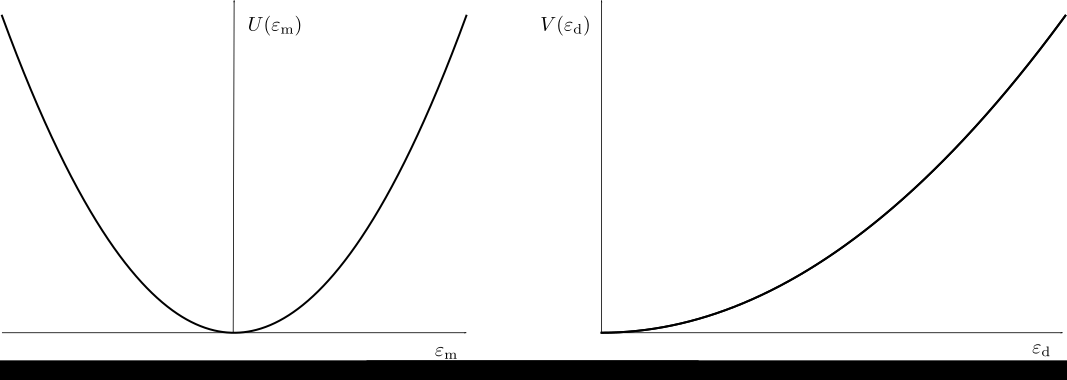
\includegraphics[width=1.\textwidth]{figures/potential_U-V_elas}
  \caption{Strain energy $W ( \T{\varepsilon} ) = U ( \varepsilon_\mathrm{m} ) + V ( \varepsilon_\mathrm{d} )$ for linear elasticity.}
  \label{fig:U-V:elas}
\end{figure}

\begin{figure}[htp]
  \centering
  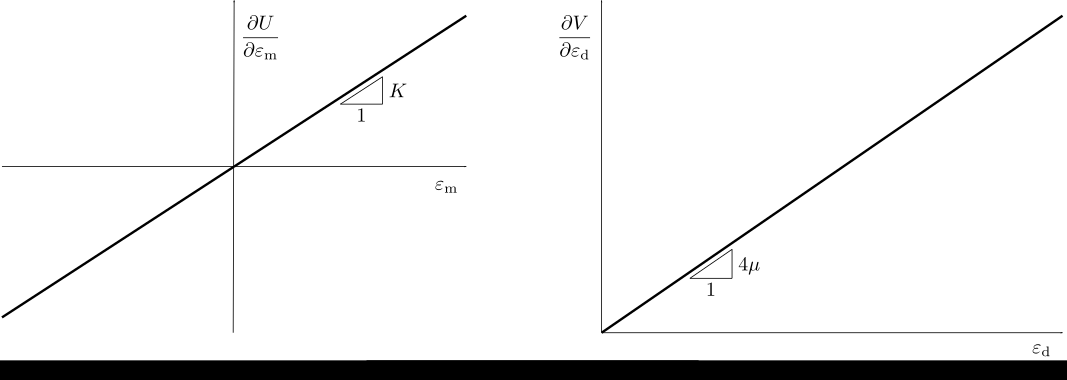
\includegraphics[width=1.\textwidth]{figures/potential_dU-dV_elas}
  \caption{Derivative of the hydrostatic strain energy $U$ and the deviatoric strain energy $V$ w.r.t.\ respectively the hydrostatic strain $\varepsilon_\mathrm{m}$ and the equivalent deviatoric strain $\varepsilon_\mathrm{d}$.}
  \label{fig:dU-dV:elas}
\end{figure}

\subsection{Plastic potential -- Parabolic potential with multiple minima}

The model is now extended to account for plasticity. The model is defined such that the material responds volumetrically purely elastic, while in shear the model is governed by multiple minima. These minima have the effect that when the material reaches a certain yield stress, it jumps to the next minimum. Around this minimum the elasticity is always the same. When loading is continued the the material again jumps to a new minimum when the next yield stress is reached. The magnitude of the jumps and of the yield stress are thereby related.

As described, the volumetric behaviour is simply elastic; whereby the potential is given by Eq.~(\ref{eq:potentials:elastic}a) and is plotted in Fig.~\ref{fig:U-V:elas}(a). To attain the desired behaviour in shear, the equivalent deviatoric strain space is divided in a finite number of yield strains $\varepsilon_\mathrm{y}^{(0)}, \varepsilon_\mathrm{y}^{(1)}, \varepsilon_\mathrm{y}^{(2)}, ...$. A parabolic potential is then defined between each pair ($[ \varepsilon_\mathrm{y}^{(0)}, \varepsilon_\mathrm{y}^{(1)} )$, $[ \varepsilon_\mathrm{y}^{(1)}, \varepsilon_\mathrm{y}^{(2)} )$, ...).

The shear strain energy is then composed of a manifold of quadratic contributions
\begin{equation}\label{eq:V-plas}
  V \big(
    \varepsilon_\mathrm{y}^{(i)} \leq \varepsilon_\mathrm{d} < \varepsilon_\mathrm{y}^{(i+1)}
  \big)
  =
  V^{(i)}
  =
  2 \mu \, \bigg[\,
    \Big[\, \varepsilon_\mathrm{d} - \varepsilon_\mathrm{min}^{(i)} \,\Big]^2
    -
    \Big[\, \Delta \varepsilon_\mathrm{y}^{(i)} \,\Big]^2
  \,\bigg]
\end{equation}
where the mean of $\varepsilon_\mathrm{y}^{(i)}$ and $\varepsilon_\mathrm{y}^{(i+1)}$ is
\begin{equation}
  \varepsilon_\mathrm{min}^{(i)}
  =
  \frac{1}{2} \Big[\, \varepsilon_\mathrm{y}^{(i+1)} + \varepsilon_\mathrm{y}^{(i)} \,\Big]
\end{equation}
which is also the equivalent deviatoric strain at which the shear strain energy reaches its minimum. It may be interpreted as a plastic strain. From this minimum, the distance to $\varepsilon_\mathrm{y}^{(i)}$ and $\varepsilon_\mathrm{y}^{(i+1)}$ is
\begin{equation}
  \Delta \varepsilon_\mathrm{y}^{(i)}
  =
  \frac{1}{2} \Big[\, \varepsilon_\mathrm{y}^{(i+1)} - \varepsilon_\mathrm{y}^{(i)} \,\Big]
\end{equation}
The resulting shear strain energy is plotted in Fig.~\ref{fig:V:plas}(a).

The stress response is obtained using
\begin{equation}\label{eq:dV-plas}
  \frac{\partial V^{(i)}}{\partial \varepsilon_\mathrm{d}}
  =
  4 \mu \, \Big[\, \varepsilon_\mathrm{d} - \varepsilon_\mathrm{min}^{(i)} \,\Big]
\end{equation}
(see Fig.~\ref{fig:dV:plas}(a)). From which it can be observed that in elasticity the behaviour is identical to above (cf.~(\ref{eq:potentials:elastic}b)). For the case that $\varepsilon_\mathrm{y}^{(0)} = - \varepsilon_\mathrm{y}^{(1)}$ the responses are even identical until initial yield stress is reached. For completeness, the stress reads
\begin{equation}
  \T{\sigma} ( \T{\varepsilon} )
  =
  K \, \text{tr} ( \T{\varepsilon} ) \, \T{I}
  +
  2 \mu \, \Big[\, \varepsilon_\mathrm{d} - \varepsilon_\mathrm{min}^{(i)} \,\Big] \;
  \T{N}_\mathrm{d}
  \qquad
  \mathrm{for}
  \;
  \varepsilon_\mathrm{y}^{(i)} \leq \varepsilon_\mathrm{d} < \varepsilon_\mathrm{y}^{(i+1)}
\end{equation}
whereby one has to assume that when $\varepsilon_\mathrm{d} = 0$ also $\T{\sigma}_\mathrm{d} = \T{0}$ in order to avoid zero division. The response is plotted in Fig.~\ref{fig:dV:plas}(a), from which it is observed that it exhibits stress jumps between different parabola in the potential, because of the discontinuity in the second derivative of the elastic potential. This can be remedied, such as in the model presented below.

\subsection{Plastic potential -- Smooth parabolic potential with multiple minima}

The remedy the discontinuity in the second derivative of the potential, it is smoothened as follows:
\begin{equation}\label{eq:V-plas-smooth}
  V \big(
    \varepsilon_\mathrm{y}^{(i)} \leq \varepsilon_\mathrm{d} < \varepsilon_\mathrm{y}^{(i+1)}
  \big)
  =
  V^{(i)}
  =
  - 4 \mu \,
  \left[ \frac{\Delta \varepsilon_\mathrm{y}^{(i)}}{\pi} \right]^2
  \left[
    1
    +
    \cos \left(
      \frac{ \pi }{ \Delta \varepsilon_\mathrm{y}^{(i)} }
      \Big[\, \varepsilon_\mathrm{d} - \varepsilon_\mathrm{min}^{(i)} \,\Big]
    \right)
  \right]
\end{equation}
which is plotted in Fig.~\ref{fig:V:plas}(b). In this case the stress is obtained from
\begin{equation}\label{eq:dV-plas-smooth}
  \frac{\partial V^{(i)}}{\partial \varepsilon_\mathrm{d}}
  =
  4 \mu \,
  \left[ \frac{\Delta \varepsilon_\mathrm{y}^{(i)}}{\pi} \right]
  \sin \left(
    \frac{ \pi }{ \Delta \varepsilon_\mathrm{y}^{(i)} }
    \Big[\, \varepsilon_\mathrm{d} - \varepsilon_\mathrm{min}^{(i)} \,\Big]
  \right)
\end{equation}
(see Fig.~\ref{fig:dV:plas}(b)). Which is to the first order equal to linear elasticity around its minimum $\varepsilon_\mathrm{min}^{(i)}$. Indeed, the first order Taylor series of Eq.~\eqref{eq:dV-plas-smooth} around $\varepsilon_\mathrm{d} = \varepsilon_\mathrm{min}^{(i)}$,
\begin{equation}
  \frac{\partial V^{(i)}}{\partial \varepsilon_\mathrm{d}}
  \approx
  4 \mu \, \Big[\, \varepsilon_\mathrm{d} - \varepsilon_\mathrm{min}^{(i)} \,\Big]
\end{equation}
is identical to Eq.~\eqref{eq:dV-plas}.

For completeness, also in case the expression for the entire stress tensor
\begin{equation}
  \T{\sigma} ( \T{\varepsilon} )
  =
  K \, \text{tr} ( \T{\varepsilon} ) \, \T{I}
  +
  2 \mu \,
  \left[ \frac{\Delta \varepsilon_\mathrm{y}^{(i)}}{\pi} \right]
  \sin \left(
    \frac{ \pi }{ \Delta \varepsilon_\mathrm{y}^{(i)} }
    \Big[\, \varepsilon_\mathrm{d} - \varepsilon_\mathrm{min}^{(i)} \,\Big]
  \right)
  \T{N}_\mathrm{d}
  \qquad
  \mathrm{for}
  \;
  \varepsilon_\mathrm{y}^{(i)} \leq \varepsilon_\mathrm{d} < \varepsilon_\mathrm{y}^{(i+1)}
\end{equation}
whereby, again, one has to assume that when $\varepsilon_\mathrm{d} = 0$ also $\T{\sigma}_\mathrm{d} = \T{0}$ in order to avoid zero division.

\begin{figure}[htp]
  \centering
  \includegraphics[width=1.\textwidth]{figures/potential_V-plas}
  \caption{The multi-minima shear strain energy, $V ( \varepsilon_\mathrm{d} )$, that models the effect of plasticity. The multi-parabolic shear strain energy is shown in (a), while its smoothened equivalent is shown in (b).}
  \label{fig:V:plas}
\end{figure}

\begin{figure}[htp]
  \centering
  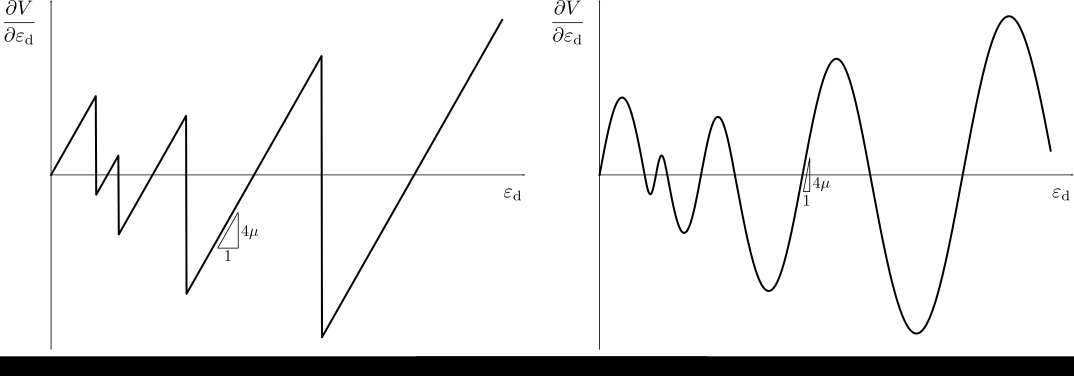
\includegraphics[width=1.\textwidth]{figures/potential_dV-plas}
  \caption{Derivative of the shear strain energy $V$.}
  \label{fig:dV:plas}
\end{figure}

\section{Nomenclature}
\label{sec:nomenclature}

\subsection{Tensors and tensor products}
\label{sec:nomenclature:tensor}

\begin{itemize}
%
\item Second order tensor
\begin{equation}
  \T{A} = A_{ij} \vec{e}_i \vec{e}_j
\end{equation}
%
\item Dyadic tensor product
\begin{align}
  \T{C} &= \vec{a} \otimes \vec{b} \\
  C_{ij} &= a_{i} \, b_{j}
\end{align}
%
\item Double tensor contraction
\begin{align}
  C &= \T{A} : \T{B} = \text{tr} \left( \T{A} \cdot \T{B} \right) \\
    &= A_{ij} \, B_{ji}
\end{align}
%
\end{itemize}

\subsection{Unit tensors}
\label{sec:nomenclature:unit}

\begin{itemize}
%
\item Second order unit tensor
\begin{equation}
  \T{I} = \delta_{ij} \vec{e}_i \vec{e}_j
\end{equation}
It is easy to show that it has the property that
\begin{equation}
  \T{I} : \T{A} = \text{tr} ( \bm{A} )
\end{equation}
%
\item Fourth order unit tensor:
\begin{equation}
  \TT{I} : \T{A} \equiv \T{A}
\end{equation}
i.e.
\begin{equation}
  \delta_{il} \delta_{jk} A_{lk} = A_{ij}
\end{equation}
hence
\begin{equation}
  \TT{I} = \delta_{il} \delta_{jk} \vec{e}_i \vec{e}_j \vec{e}_k \vec{e}_l
\end{equation}
%
\item Deviatoric projection
\begin{equation}
  \TT{I}_\mathrm{d} : \T{A} \equiv \T{A} - \tfrac{1}{3} \text{tr} ( \bm{A} ) \T{I}
\end{equation}
hence
\begin{equation}
  \TT{I}_\mathrm{d} = \TT{I} - \tfrac{1}{3} \T{I} \otimes \T{I}
  = \left( \delta_{il} \delta_{jk} - \tfrac{1}{3} \delta_{ij} \delta_{kl} \right) \vec{e}_i \vec{e}_j \vec{e}_k \vec{e}_l
\end{equation}
%
\end{itemize}


\subsection{Strain measures}
\label{sec:nomenclature::strain}

\begin{itemize}
%
\item Strain deviator
\begin{equation}
  \T{\varepsilon}_\mathrm{d}
  = \T{\varepsilon} - \tfrac{1}{3} \text{tr} ( \T{\varepsilon} ) \, \T{I}
  = \TT{I}_\mathrm{d} : \T{\varepsilon}
\end{equation}
%
\item Equivalent deviatoric strain
\begin{equation}
  \varepsilon_\mathrm{d}
  = \; \sqrt{
    \tfrac{1}{2} \, \T{\varepsilon}_\mathrm{d} : \T{\varepsilon}_\mathrm{d}
  }
\end{equation}
%
\end{itemize}

\subsection{Stress measures}
\label{sec:nomenclature::stress}

\begin{itemize}
%
\item Stress deviator
%
\begin{equation}
  \T{\sigma}_\mathrm{d}
  = \T{\sigma} - \tfrac{1}{3} \text{tr} ( \T{\sigma} ) \, \T{I}
  = \TT{I}_\mathrm{d} : \T{\sigma}
\end{equation}
%
\item Equivalent deviatoric stress
\begin{equation}
\sigma_\mathrm{d} = \sqrt{ 2 \, \T{\sigma}_\mathrm{d} : \T{\sigma}_\mathrm{d} }
\end{equation}
Note that this definition is such that the equivalent deviatoric stress and strain are work conjugate, i.e.
\begin{equation}
  \T{\sigma} : \T{\varepsilon} = \sigma_\mathrm{d} \varepsilon_\mathrm{d}
\end{equation}
%
\end{itemize}

\subsection{Derivatives}
\label{sec:nomenclature:derivatives}

\begin{itemize}
%
\item Trace of the strain
\begin{equation}
  \frac{ \partial \, \text{tr} ( \T{\varepsilon} ) }{ \partial \T{\varepsilon} }
  =
  \frac{ \partial }{ \partial \T{\varepsilon} } \left( \T{\varepsilon} : \T{I} \right)
  =
  \frac{ \partial \T{\varepsilon} }{ \partial \T{\varepsilon} } : \T{I}
  =
  \TT{I} : \T{I}
  =
  \T{I}
\end{equation}
%
\item Strain deviator
\begin{equation}
  \frac{ \partial \T{\varepsilon}_\mathrm{d} }{ \partial \T{\varepsilon} }
  =
  \frac{ \partial }{ \partial \T{\varepsilon} } \left( \T{\varepsilon} - \tfrac{1}{3} \text{tr} ( \T{\varepsilon} ) \T{I} \right)
  =
  \TT{I} - \tfrac{1}{3} \T{I} \otimes \T{I}
  =
  \TT{I}_\mathrm{d}
\end{equation}
%
\item Equivalent shear strain
\begin{equation}
  \frac{ \partial \varepsilon_\mathrm{d} }{ \partial \T{\varepsilon} }
  =
  \frac{1}{2 \, \varepsilon_\mathrm{d}} \frac{1}{2}
  \big[\, \TT{I}_\mathrm{d} : \T{\varepsilon}_\mathrm{d} + \T{\varepsilon}_\mathrm{d} : \TT{I}_\mathrm{d} \,\big]
  =
  \frac{\T{\varepsilon}_\mathrm{d}}{2 \, \varepsilon_\mathrm{d}}
  \equiv
  \tfrac{1}{2} \T{N}_d
\end{equation}
%
\end{itemize}

% \section{Specialized model -- planar shear}

% \subsection{Motivation}

% The model as proposed above treats all shear modes equally (because $V$ is function of $\varepsilon_\mathrm{d}$). Consequently it is isotropic. There are, however, cases for which an anisotropic model is more realistic. Below a model is proposed in which the plasticity can only occur along a specific plane. Before that, the claim of isotropy is further motivated in two dimensions. In that case the strain tensor has three independent modes, illustrated in Fig.~\ref{fig:strain-modes:2d}.

% \begin{figure}[htp]
%   \centering
%   \includegraphics[width=.7\textwidth]{figures/strain-modes_2d}
%   \caption{The three independent modes described by a 2-d stain tensor $\T{\varepsilon}$.}
%   \label{fig:strain-modes:2d}
% \end{figure}

% The first shear mode, in Fig.~\ref{fig:strain-modes:2d}(b), corresponds to a strain tensor of the following structure
% \begin{equation} \label{eq:strain-modes:basic}
%   \underline{\underline{\varepsilon}}
%   =
%   \begin{bmatrix}
%     0      & \gamma \\
%     \gamma &  0
%   \end{bmatrix}
% \end{equation}
% The second shear mode, in Figure~\ref{fig:strain-modes:2d}(c), corresponds to the same shear deformation rotated by $-\pi/4$. It is therefore of the structure
% \begin{equation}
%   \underline{\underline{\varepsilon}}
%   =
%   \begin{bmatrix}
%     \gamma &  0      \\
%      0     & -\gamma
%   \end{bmatrix}
% \end{equation}

% In terms of the equivalent deviatoric strain, both modes result in $\varepsilon_\mathrm{d} = | \gamma |$. This is further illustrated by rotating the strain tensor from Eq.~\eqref{eq:strain-modes:basic} by an angle $\theta$:
% \begin{equation}
%   \underline{\underline{\varepsilon}}^\prime
%   =
%   \underline{\underline{R}} \,
%   \underline{\underline{\varepsilon}} \,
%   \underline{\underline{R}}^T
% \end{equation}
% where the rotation matrix depends on the rotation angle $\theta$ as follows
% \begin{equation}
%   \underline{\underline{R}}
%   =
%   \begin{bmatrix}
%     \cos \theta & - \sin \theta \\
%     \sin \theta &   \cos \theta
%   \end{bmatrix}
% \end{equation}
% Trivially $\varepsilon_\mathrm{d} = | \gamma |$, independent of $\theta$ -- as plotted in Fig~\ref{fig:shear-modes:epseq} in black. The contributions of the two shear modes are examined by examining $\varepsilon^\prime_{xy}$, representative of the first shear mode in Fig.~\ref{fig:strain-modes:2d}(b), and $\varepsilon^\prime_{xx}$, representative of the second shear mode in Fig.~\ref{fig:strain-modes:2d}(c). These contributions are plotted in Fig.~\ref{fig:shear-modes:epseq} respectively in green and red. Indeed, the contributions of the two shear modes vary with $\theta$, while $\varepsilon_\mathrm{d}$ it is oblivious to this rotation.

% \begin{figure}[htp]
%   \centering
%   \includegraphics[width=.5\textwidth]{figures/strain-modes_2d_epseq}
%   \caption{Comparison between the equivalent deviatoric strain $2 \varepsilon_\mathrm{d}^2 = \T{\varepsilon}_\mathrm{d} : \T{\varepsilon}_\mathrm{d}$ the strain along the $x$-plane, $\varepsilon_\mathrm{ss} = \vec{e}_x \cdot \T{\varepsilon} \cdot \vec{e}_y$, and the strain perpendicular to it, $\varepsilon_\mathrm{ps} = \vec{e}_x \cdot \T{\varepsilon} \cdot \vec{e}_x$.}
%   \label{fig:shear-modes:epseq}
% \end{figure}

% \subsection{Model}

% In this model, the plasticity will be localised on a plane with normal $\vec{n}$ (which has unit length $||\, \vec{n} \,|| \equiv 1$), see Fig.~\ref{fig:strain-vector-planar}. To do so, the strain deviator $\T{\varepsilon}_\mathrm{d}$ is decomposed in two parts, the strain along the plastic (`weak') plane $\T{\varepsilon}_\mathrm{s}$, and the remaining strain $\T{\varepsilon}_\mathrm{n}$. I.e.
% \begin{equation}\label{eq:planar:strain:decomposition}
%   \T{\varepsilon}_\mathrm{d} = \T{\varepsilon}_\mathrm{s} + \T{\varepsilon}_\mathrm{n}
% \end{equation}
% To compute the former, planar strain tensor $\T{\varepsilon}_\mathrm{s}$, first the direction of the deviatoric stain tensor projected on the plane is determined as
% \begin{equation}
%   \vec{s}_\mathrm{n} =
%   \frac{
%     \T{\varepsilon}_\mathrm{d} \cdot \vec{n}
%   }
%   {
%     ||\, \T{\varepsilon}_\mathrm{d} \cdot \vec{n} \,||
%   }
% \end{equation}
% The strain direction along the plane is now found by projecting $\vec{s}_\mathrm{n}$ on it:
% \begin{equation}
%   \vec{s} =
%   \frac{
%     \vec{s}_\mathrm{n} - ( \vec{s}_\mathrm{n} \cdot \vec{n} )\, \vec{n}
%   }
%   {
%     ||\, \vec{s}_\mathrm{n} - ( \vec{s}_\mathrm{n} \cdot \vec{n} )\, \vec{n} \,||
%   }
% \end{equation}
% The amount of strain in this direction is finally found to be
% \begin{equation}
%   \varepsilon_\mathrm{s} = \vec{s} \cdot \T{\varepsilon}_\mathrm{d} \cdot \vec{n}
% \end{equation}
% Not that $\varepsilon_\mathrm{s}$ is by definition non-negative, i.e.\ it is oblivious to rotations about $\vec{n}$.

% The planar deviatoric strain tensor can now be constructed:
% \begin{equation}
%   \T{\varepsilon}_\mathrm{s} = \varepsilon_\mathrm{s}
%   \big(
%     \vec{s} \otimes \vec{n} + \vec{n} \otimes \vec{s}
%   \big)
% \end{equation}
% From this it is obvious that $\varepsilon_\mathrm{s}$ is the equivalent deviatoric strain of this tensor, i.e.
% \begin{equation}
%   \varepsilon_\mathrm{s}
%   \equiv
%   \sqrt{ \tfrac{1}{2} \T{\varepsilon}_\mathrm{s} : \T{\varepsilon}_\mathrm{s} }
% \end{equation}
% (To show this one has to use that $\vec{n} \cdot \vec{n} \equiv 1$ and $\vec{s} \cdot \vec{s} \equiv 1$ while $\vec{n} \cdot \vec{s} \equiv 0$).

% \begin{figure}[htp]
%   \centering
%   \includegraphics[width=.35\textwidth]{figures/strain-vector-planar}
%   \caption{Strain along a plane defined by its normal $\vec{n}$: the strain vector $\vec{s}_\mathrm{n}$ and its planar projection $\vec{s}$.}
%   \label{fig:strain-vector-planar}
% \end{figure}

% The remaining strain can now be trivially obtained from Eq.~\eqref{eq:planar:strain:decomposition} as
% \begin{equation}
%   \T{\varepsilon}_\mathrm{n} = \T{\varepsilon}_\mathrm{d} - \T{\varepsilon}_\mathrm{s}
% \end{equation}
% Its equivalent deviatoric strain reads
% \begin{equation}
%   \varepsilon_\mathrm{n} = \sqrt{ \tfrac{1}{2} \T{\varepsilon}_\mathrm{n} : \T{\varepsilon}_\mathrm{n} }
% \end{equation}

% For plasticity to occur only along the `weak' plane, the shear strain energy is further decomposed in a planar part $V_\mathrm{s}$ that will be plastic, and a non-planar part $V_\mathrm{n}$ that will be elastic:
% \begin{equation}
%   V
%   =
%   V_\mathrm{s} ( \varepsilon_\mathrm{s} )
%   +
%   V_\mathrm{n} ( \varepsilon_\mathrm{n} )
% \end{equation}
% Based on the definitions of the elastic and plastic potentials the following expression for the stress is obtained
% \begin{equation}
%   \T{\sigma} ( \T{\varepsilon} )
%   =
%   K \, \varepsilon_\mathrm{m} \, \T{I}
%   +
%   2 \mu \, \T{\varepsilon}_\mathrm{n}
%   +
%   2 \mu \,
%   \left[ \frac{\Delta \varepsilon_\mathrm{y}^{(i)}}{\pi} \right]
%   \sin \left(
%     \frac{ \pi }{ \Delta \varepsilon_\mathrm{y}^{(i)} }
%     \Big[\, \varepsilon_\mathrm{s} - \varepsilon_\mathrm{min}^{(i)} \,\Big]
%   \right)
%   \frac{\T{\varepsilon}_\mathrm{s}}{\varepsilon_\mathrm{s}}
%   \quad
%   \mathrm{for}
%   \;
%   \varepsilon_\mathrm{y}^{(i)} \leq \varepsilon_\mathrm{s} < \varepsilon_\mathrm{y}^{(i+1)}
% \end{equation}


\bibliography{library}

\end{document}
